\documentclass[main.tex]{subfiles}
\begin{document}


\chapter{Differentialrechnung}


\begin{Bemerkung}
  Im Moment beschränken wir uns auf reellwertige Funktionen in einer Variable (also $\R^1 \to \C$), definiert auf offenen Intervallen.
\end{Bemerkung}


\section{Ableitung und Ableitungsregeln}

\begin{Definition}[Differenzierbarkeit]
  Seien $a < b \in \R$, sei $f:(a,b) = D \to \C$ eine Funktion und $x_0 \in (a,b)$. Wir sagen $f$ sei \textbf{differenzierbar} bei $x_0$ falls der Grenzwert
  $$f'(x_0) = \lim \limits_{\substack{x \to x_0 \\ x \neq x_0}} \dfrac{f(x)-f(x_0)}{x - x_0} = \lim \limits_{h\to 0} \dfrac{f(x_0+h)-f(x_0)}{h}$$
  existiert.

  Wir sagen $f$ sei differenzierbar auf $(a,b)$ falls $f$ in jedem Punkt $x_0 \in (a,b)$ differenzierbar ist. In diesem Fall nennen wir $f':(a,b) \to \C$ die \text{Ableitung} von $f$.
\end{Definition}


\begin{Bemerkung}
  Diese Definition ist nur dann sinnvoll, wenn $D$ ein Intervall ist und $x_0$ ein Häufungspunkt von $D$ ist. Deshalb gehen wir im Folgenden davon aus.
\end{Bemerkung}

\begin{Bemerkung}
  Die Erweiterung der Definition von $\R$ auf $\C$ ist einfach, denn es genügt, den Real- und Imaginärteil von $f$ separat zu betrachten.
\end{Bemerkung}

\begin{Bemerkung}
  \begin{Theorem}
    Ist $f$ bei $x_0 \in D$ differenzierbar, so ist $f$ stetig bei $x_0$.

    Diese Aussage lässt sich verallgemeinern:
    $$f \text{ ist differenzierbar} \Rightarrow f \text{ ist stetig}$$
  \end{Theorem}
  \begin{Beweis}
    $$\lim \limits_{\substack{x \to x_0 \\ x \neq x_0}}|f(x)-f(x_0)| = \underbrace{\limx |x - x_0|}_{=0} \cdot \underbrace{\limx \dfrac{|f(x)-f(x_0)|}{|x - x_0}}_{= |f'(x_0)|} = 0$$
  \end{Beweis}
\end{Bemerkung}

\begin{Bemerkung}[alternative Notationen]
  \begin{itemize}
    \item $\dfrac{d}{dx}f(x)$
    \item $\dfrac{d}{d x} f$
    \item $D f, df$
    \item $f_x$
    \item $f^{(1)}$
    \item Und auch die links- und rechtsseitigen Ableitungen mit $x < x_0$ und $x > x_0$.
  \end{itemize}
\end{Bemerkung}

\begin{Beispiel}
  \begin{itemize}
    \item Nein, den Fall $ax + b$ werde ich ganz sicher nicht abschreiben...
    \item $D = \R$, $f: D \to \C$, $c \in \C$ gegeben durch: $f(x) = \exp(c \cdot x)$.

      Wähle $x_0 \in \R$:
      $$\begin{aligned}
        f'(x_0) = \lim \limits_{h\to0} \dfrac{f(x_0+h)-f(x_0)}{h}
        &= \lim \limits_{h\to 0} \dfrac{\exp(cx_0 + ch)-\exp(cx_0)}{h} \\
        &= \exp(c x_0) \cdot \lim \limits_{h \to 0} \dfrac{\exp(ch)-1}{h} \\
        &= \exp(c x_0) \cdot \lim \limits_{h \to 0} \dfrac{1}{n}\sum \limits_{n=0}^\infty \dfrac{(ch)^n}{n!} \\
        &= \exp(c x_0) \cdot \lim \limits_{h \to 0} \sum \limits_{n=1}^\infty \dfrac{(ch)^n}{n!} \\
        &= \exp(c x_0) \cdot \lim \limits_{h \to 0} \sum \limits_{n=1}^\infty \dfrac{c^n}{n!}h^{n-1} \\
        & \underbrace{\text{Konvergenzradius = }\infty}_{\text{stetige Funktion von }h} \\
        &= \exp(c x_0) \cdot c
      \end{aligned}$$
    \item $D = \R \backslash\{0\}$, $f: D \to \C$ gegeben durch: $f(x) = \dfrac{1}{x}$.
      $$\begin{aligned}
        f'(x_0) = \lim \limits_{h\to0} \dfrac{\frac{1}{x_0+h}-\frac{1}{x_0}}{h} &= \lim \limits_{h\to 0} \dfrac{-(x_0 + h)+x_0}{(x_0 +h) x_0 h}\\
        &= \lim \limits_{h\to0} \dfrac{-1}{(x_0+h)x_0}\\
        &= -\dfrac{1}{x_0^2}
      \end{aligned}$$
  \end{itemize}
\end{Beispiel}

\begin{Theorem}
  $$(\exp(c\cdot x_0))' = \exp(c x_0) \cdot c$$
  Konsequenz (Sonderfall $c = i$):
  $$(\sin(x))' = \cos(x) \quad (\cos(x))' = -\sin(x)$$
\end{Theorem}

\begin{Theorem}
  Seien $f,g: D \to \R$ differenzierbar an der Stelle $x_0 \in D$. Dann sind $f+g$ und $f\cdot g$ ebenfalls differenezierbar bei $x_0$ und es gilt:
  \begin{itemize}
    \item $(f+g)'(x_0) = f'(x_0) + g'(x_0)$
    \item Leibnitz-Regel: $(f\cdot g)'(x_0) = f'(x_0) \cdot g(x_0) + f(x_0) \cdot g'(x_0)$
  \end{itemize}
\end{Theorem}

\begin{Beweis}
  \begin{itemize}
    \item Additivität von Grenzwerten.
    \item Auch hier kommt uns die Additivität entgegen:
      $$\begin{aligned}
      (f \cdot g)'(x_0)&  = \limx \dfrac{f(x)g(x) - f(x_0)g(x_0)}{x-x_0}\\
      & = \limx \dfrac{f(x)g(x) - f(x_0)g(x) + f(x_0)g(x) - f(x_0)g(x_0)}{x-x_0}\\
      & = \limx \dfrac{f(x)g(x) - f(x_0)g(x)}{x-x_0} + \limx \dfrac{f(x_0)g(x) - f(x_0)g(x_0)}{x-x_0}\\
      & = \limx \underbrace{g(x)}_{\to g(x_0)} \dfrac{f(x) - f(x_0)}{x-x_0} + \limx \underbrace{f(x_0)}_{\text{konstant}} \dfrac{g(x) - g(x_0)}{x-x_0}\\
      & = g(x_0)f'(x_0) + f(x_0)g'(x_0)
    \end{aligned}$$
  \end{itemize}
\end{Beweis}

\begin{Bemerkung}[Konsequenz]
  $f(x) = x$, $f: \R \to \R$, $f'(x) = 1$.

  Sei $g(x) = x^2 = f \cdot f$, also gilt: $f'(x) = (f \cdot f)'(x) = f'f + ff' = 2ff' = 2x$.

  Allgemeiner gilt für $h(x) = x^n, n \geq 0$: $h'(x) = n \cdot x^{n-1}$ (Induktion).
\end{Bemerkung}

Noch allgemeiner gilt:

\begin{Theorem}
  Sei $P: \R \to \C$ gegeben durch:
  $$P(x) = \sum \limits_{n = 0}^\infty a_n x^n$$
  mit $a_n \in \C$, dann gilt:
  $$P'(x) = \sum \limits_{n = 0}^\infty n \cdot a_n x^{n-1}$$
\end{Theorem}

Außerdem nützlich:
\begin{Theorem}[Kettenregel]
  Seien $D, E \subseteq \R$ offen. Seien $f: D \to E$, $g: D \to \R$ differenzierbar. Die Funktion
  $$(g \circ f) = g(f): D \to \R$$
  ist differenzierbar und es gilt:
  $$ (g \circ f)'(x_0) = g'(f(x_0)) \cdot f'(x_0)$$
\end{Theorem}

\begin{Beweis}
  Wichtig, also live verfolgt. Siehe Skript.
\end{Beweis}

\begin{Beispiel}
  Sei $f : D \to \R\backslash\{0\}$ differenzierbar. Dann ist $h: D \to \R$ gegeben durch $h(x) = \dfrac{1}{f(x)}$ ebenfalls differenzierbar und es gilt
  $$h'(x) = \left(\dfrac{1}{f}\right)(x) = - \dfrac{1}{f(x)^2}f'(x)$$
\end{Beispiel}

Allgemeiner folgt:
\begin{Theorem}[Quotientenregel]
  Seien $f,g:D\to \R$ differenzierbar an der Stelle $x_0 \in D$ und sei $g(x_0) \neq 0$. Dann ist $h(x) = \dfrac{f(x)}{g(x)}$ ebenfalls differenezierbar bei $x_0$ und es gilt:
  $$h'(x_0) = \left(\dfrac{f(x_0)}{g(x_0)}\right)' = \dfrac{f'(x_0)g(x_0) - f(x_0)g'(x_0)}{g^2(x_0)}$$
\end{Theorem}

\begin{Theorem}[Inversenregel]
  Seien $D,E \subseteq \R$ offen und $f: D \to E$ bijektiv und differenzierbar. Sei $g = f^{-1} : E \to D$ stetig.

  Ist $x_0 \in D$, so dass $f'(x_0) \neq 0$, so ist $g$ bei $f(x_0) = y_0$ ableitbar, und es gilt:
  $$g'(y_0) = \dfrac{1}{f'(x_0)}$$
\end{Theorem}

\begin{Beweis}
  $$g'(y_0) = \lim \limits_{y \to y_0} \dfrac{g(y)-g(y_0)}{y - y_0} = \limx \dfrac{g(f(x))-g(f(x_0))}{f(x) - f(x_0)} = \limx \dfrac{x - x_0}{f(x) - f(x_0)} = \dfrac{1}{f'(x_0)}$$
\end{Beweis}

\begin{Beispiel}
  $D = \R$, $E = \R_{> 0}$, $f: D \to E$, $f(x) = \exp(x) \Rightarrow g(y) = \log(y)$.

  Sei $x_0 = \exp(x_0) \in \R_{>0}$ und $x_0 = \log(y_0)$
  $$g'(y_0) = \dfrac{1}{f'(x_0)} = \dfrac{1}{\exp(\log(y_0))} = \dfrac{1}{y_0}$$
  $\Rightarrow \log'(y) = \dfrac{1}{y}$
\end{Beispiel}

\begin{Definition}[Glatte Funktionen]
  Sei $D \subseteq \R$ ohne isolierte Punkte. Dann bezeichnen wir
  $$\mathcal{C}(D) = C^0(D)$$
  als alle stetigen reellwertigen Funktionen auf $D$,
  $$\mathcal{C}^1(D)$$
  als den Vektorraum aller differenzierbaren Funktionen auf $D$, deren Ableitung stetig ist. (diese Funktionen nennen wir stetig differenzierbar).

  Für $n \geq 1$ definiere rekursiv:
  $$\mathcal{C}^n(D)$$
  den Vektorraum aller differenzierbaren Funktionen $f$ auf $D$ mit $f' \in C^{n-1}(D)$.
  $$\mathcal{C}^\infty(D)=\bigcap_{n=0}^\infty \mathcal{C}^n(D)$$
  Wir nennen $f \in \mathcal{C}^\infty (D)$ \textbf{glatte Funktion}.
\end{Definition}

\begin{Beispiel}
  \begin{itemize}
    \item $\exp$
    \item $\sin, \cos$
    \item $\log$
    \item Polynome
    \item $f(x) = 0$ (Neutrales Element des Vektorraums)
  \end{itemize}
  sind glatt.

  Wir definieren $f:\R \to \R$ durch
  $$f(x) = \left\{\begin{aligned}
    &x^2\cdot \sin\left(\dfrac{1}{x}\right) & \text{ falls } x \neq 0\\
    &0 & \text{ falls } x = 0
  \end{aligned}\right.$$
  \begin{center}
    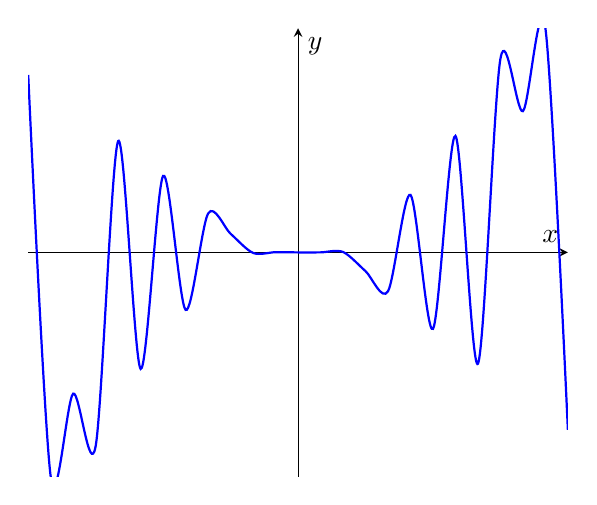
\begin{tikzpicture}
      \begin{axis}[
        domain=-0.01:0.01,
        axis x line = center,
        ticks = none,
        % ytick = none,
        axis y line = center,
        xlabel={$x$},
        ylabel={$y$},
        ]
        \addplot[smooth,color=blue,thick] {x * x * sin(deg(1/x))};
      \end{axis}
    \end{tikzpicture}
  \end{center}

  Diese Funktion ist differenzierbar auf ganz $\R$ aber \textbf{nicht} von Klasse $C^1$, d.h. $f'$ ist nicht stetig.

  Für $x \neq 0$ gilt:
  $$f'(x) = 2x \sin\left(\dfrac{1}{x}\right) + x^2 \cdot \cos\left(\dfrac{1}{x}\right) \cdot \dfrac{-1}{x^2} = 2x \sin\left(\dfrac{1}{x}\right) +\ cos\left(\dfrac{1}{x}\right)$$
  $$f'(0) = \lim \limits_{x \to 0} \dfrac{x^2 \sin\left(\frac{1}{x}\right)}{x} = \lim \limits_{x \to 0} x \sin\left(\dfrac{1}{x}\right) = 0$$
  $f''$ existiert nicht!
\end{Beispiel}


\section{Hauptsätze der Differentialrechnung}

\subsection{Extrema}

\begin{Definition}[Lokale Maxima]
  Sei $D \subseteq \R$, $f:D \to \R$ eine Funktion. Wir nennen $x_0 \in D$ \textbf{lokales Maximum} von $f$ falls
  $$\E \varepsilon > 0 : f(x) \leq f(x_0) \A x \in (x_0 - \varepsilon, x_0 + \varepsilon) \cap D$$
  $x_0$ heißt \textbf{isoliertes lokales Maximum} falls
  $$\E \varepsilon > 0 : f(x) < f(x_0) \A x \in (x_0 - \varepsilon, x_0 + \varepsilon) \cap D$$
\end{Definition}

\begin{Theorem}
  Sei $D \subseteq \R$ ein Intervall. Sei $f : D \to \R$ eine Funktion und $x_0 \in D$ ein lokales Maximum oder Minimum von $f$. Dann gilt mindestens eine der folgenden Aussagen:
  \begin{enumerate}
    \item $X_0$ ist ein Randpunkt von $D$
    \item $f$ ist nicht ableitbar bei $x_0$
    \item $f$ ist ableitbar bei $x_0$ und $f'(x) = 0$
  \end{enumerate}
\end{Theorem}

\begin{Beweis}
  Angenommen 1 und 2 sind falsch: Also existiert $x_0$ im Inneren von $D$, und $f'(x_0)$ existiert, außerdem ist $x_0$ ein lokales Extremum.
  $$\begin{aligned}
    f'(x_0) = \lim \limits_{\substack{x \to x_0 \\ x \neq x_0}} \dfrac{f(x) - f(x_0)}{x - x_0}
    &=\lim \limits_{\substack{x \to x_0 \\ x > x_0}} \dfrac{\overbrace{f(x) - f(x_0)}^{\leq 0}}{\underbrace{x - x_0}_{>0}} \leq 0\\
    &= \lim \limits_{\substack{x \to x_0 \\ x < x_0}} \dfrac{\overbrace{f(x) - f(x_0)}^{\leq 0}}{\underbrace{x - x_0}_{<0}} \geq 0\\
    &= 0
  \end{aligned}$$
\end{Beweis}

\subsection{Mittelwertsatz}

Wir haben verschiedene Formulierungen:

Satz von Rolle:
\begin{Theorem}[Mittelwertsatz]
  Sei $D \subseteq \R$ ein Intervall, $f : D \to \R$ ableitbar, $a<b \in D$ mit $f(a) \leq f(b)$. Dann existiert $x \in (a,b)$ mit $f'(x) = 0$.
\end{Theorem}

\begin{Beweis}
  Da $[a,b]$ kompakt ist und $f$ stetig ist, nimmt $f$ ihr Maximum $x_2$ auf $[a,b]$ an.

  Falls $x_1 \in (a,b)$, dann ist $x_1$ ein lokales Maximum und es folgt $F'(x_1) = 0$.

  Selbes falls $x_2 \in (a,b)$.

  Falls $x_1,x_2 \in \{a,b\}$, dann gilt $f(x_1) = f(x_2)$ also ist $f$ konstant und es gilt: $f'(x) = 0 \A x \in (a,b)$
\end{Beweis}

\begin{Korollar}[Mittelwertsatz]
  Sei $D \subseteq \R$ ein Intervall, $f : D \to \R$ ableitbar, $a < b \in D$. Dann existiert $x \in (a,b)$ mit
  $$f'(x) = \dfrac{f(b)-f(a)}{b-a}$$
\end{Korollar}

\begin{Beweis}
  Definiere $g : [a,b] \to \R$ durch $g(x) = f(x) - \dfrac{f(b)-f(a)}{b-a} (x - a)$.

  $f(a) = g(a)$; $g(b) = f(a)$.

  Laut Satz von Rolle existiert ein $x \in (a,b)$ mit $g'(x) = 0$.
  $$g'(x) = f'(x) - \dfrac{f(b)-f(a)}{b-a} = 0$$
  \begin{Bemerkung}
    Anschaulich: Betrachte die Gerade durch $f(a)$ und $f(b)$. Zwischen $a$ und $b$ gibt es $x$, wo die Steigung von $f(x)$ gleich der dieser Durchschnittsgeraden sind.
    \incfig{zwischenwertsatz_2}
  \end{Bemerkung}
\end{Beweis}

Und wir haben Cauchys Version:
\begin{Korollar}[Mittelwertsatz]
  Seien $f,g : [a,b] \to \R$ differenzierbar. Dann existiert $x \in (a,b)$ mit:
  $$g'(x)(f(b) - f(a)) = f'(x)(g(b) - g(a))$$
\end{Korollar}

\begin{Beweis}
  Definiere $F : [a,b] \to \R$ durch
  $$F(x) = g(x)(f(b) - f(a)) - f(x)(g(b) - g(a))$$
  Dann gilt $F(a) = F(b)$ und also existiert $x \in (a,b)$ mit $F'(x) = 0$
\end{Beweis}

\begin{Korollar}
  Sei $D \in \R$ ein Intervall, $f: D \to \R$ ableitbar it $f'(x) = 0 \A x \in D$. Dann ist $f$ konstant.
\end{Korollar}

\begin{Bemerkung}
  Gilt nur auf einem \textbf{Intervall}! Das heißt zum Beispiel nicht auf Vereinigungen von disjunkten Intervallen.
\end{Bemerkung}

\subsection{Korollare und Kurvendiskussion}

\begin{Theorem}[Monotonie]
  Sei $D \subseteq \R$ ein Intervall, $f : D \to \R$ stetig differenzierbar. Dann gilt:
  $$f \text{ ist monoton steigend} \Leftrightarrow f'(x) \geq 0 \A x \in D$$
\end{Theorem}

\begin{Beweis}
  \begin{itemize}
    \item $\Rightarrow$: $f$ monoton steigend
      $$\Rightarrow f'(x_0) = \limx \dfrac{f(x)-f(x_0)}{x - x_0} \geq 0$$
    \item $\Leftarrow$: ist $f$ nicht monoton steigend, so gilt
     $$\E a < b \in D : f(a) > f(b) \Rightarrow \E x \in (a,b): f'(x) = \dfrac{f(b)-f(a)}{b-a} < 0 $$
     was ein Widerspruch ist.
  \end{itemize}
\end{Beweis}

\begin{Bemerkung}
  Dieser Satz gilt nicht für strenge Monotonie: $f(x)=x^3$ ist streng monoton wachsend, aber $f'(x) \not> 0 \A x \in D$. Es gilt also keine Äquivalenz. Die Folgerung vom Vorzeichen der Ableitung auf die Monotonie ist durchaus möglich.
\end{Bemerkung}

\begin{Korollar}
  Eine Funktion $f: I \to \R$ ist genau dann konstant, wenn sie differenzierbar ist und $f'(x_0) = 0 \A x_0 \in I$ gilt.
\end{Korollar}

\begin{Definition}[Konkavität und Konvexität]
  Sei $i \subseteq \R$ ein Intervall und $f:I \to \R$ eine Funktion. Dann heißt $f$ \textbf{konvex}, falls $\A a < b \in I$ und $\A t \in (0,1)$ folgende Ungleichung gilt:
  $$f((1-t)a+tb) \leq (1-t)f(a)+tf(b)$$
  \begin{itemize}
    \item Eine Funktion $g$ heißt \textbf{konkav}, wenn $f = -g$ konvex ist.
    \item Man spricht von strenger Konvexität oder Konkavität, wenn eine strikte Ungleichung vorliegt.
  \end{itemize}
\end{Definition}

\begin{Theorem}
  Sei $I \subseteq \R$ ein Intervall und $f: I \to \R$ differenzierbar. Dann ist $f$ genau dann (streng) konvex, wenn $f'$ (streng) monoton wachsend ist.
\end{Theorem}

\begin{Korollar}
  Sei $I \subseteq \R$ ein Intervall und $f: I \to \R$ 2 Mal differenzierbar. Falls $f''(x) \geq 0 \A x \in I$ ist, dann ist $f$ konvex. Bei einer strengen Ungleichung liegt strenge Konvexität vor.
\end{Korollar}

\begin{Lemma}[Jensen'sche Ungleichung]
  Sei $I \subseteq \R$ ein Intervall und $f: I \to \R$ eine konvexe Funktion. Seien $n \in \N$, $x_1,x_2,...,x_n \in I$ und $t_1, t_2, ..., t_n \in [0,1]$ mit $\sum \limits_{k=1}^n t_k = 1$. Dann gilt:
  $$f\left(\sum \limits_{k=1}^n t_k x_k\right) \leq \sum \limits_{k=1}^n t_k f(x_k)$$
\end{Lemma}

\begin{Beweis}
  Per Induktion, siehe Skript.
\end{Beweis}

\subsection{L'Hôpital}

\begin{Theorem}[Rêgle de L'Hôpital]
  Sei $D = (a,b)$ ein Intervall, $f,g : D \to \R$ differenzierbar mit $g(x) \neq 0$ und $g'(x) \neq 0 \A x \in (a,b)$. Es gelte:
  $$\lim \limits_{x \to a} f(x) = 0 \text{ und } \lim \limits_{x \to a} g(x) = 0$$
  $$\lim \limits_{x \to a} \dfrac{f'(x)}{g'(x)} = A$$
  Dann gilt:
  $$\lim \limits_{x \to a} \dfrac{f(x)}{g(x)} = A$$
\end{Theorem}

\begin{Bemerkung}
  Diese Technik funktioniert auch für Funktionen, die gegen $\pm \infty$ gehen, da man einfach die Inverse Funktion verwenden und entsprechend den inversen Grenzwert berechnet.
\end{Bemerkung}

\begin{Beweis}
  Setze $f,g$ auf $[a,b)$ fort durch $f(a) = g(a) = 0$. Sei $\varepsilon > 0$.
  $$\E \delta > 0 : \dfrac{f'(\xi)}{g'(\xi)} \in (A-\varepsilon, A + \varepsilon) \A \xi \in (a,a+\delta)$$
  Für $x \in (a, a+\delta)$ gilt nach Mittelwertsatz von Cauchy:
  $$\E \xi \in (a,b) : \dfrac{f(x)}{g(x)} = \dfrac{f(x)-f(a)}{g(x)-g(a)} = \dfrac{f'(x)}{g'(x)}$$
\end{Beweis}

\end{document}
